\section{Related Work}
\label{sec:rw}
The field of object proposals has grown rapidly and constitutes a large ever evolving body of work. Despite the vast amount of disparate literature, the area is amenable to organization by classifying methods according to how they generate object proposals and the level of output localization. If the generation process is based on thresholding a random set of image windows according to their likelihood of containing an object, then we refer to these approaches as \emph{window scoring}, Section~\ref{sec:window_scoring}. However, if the process is based on grouping low level features (pixels,superpixels, edges, etc) with the output of this merging process serving as object proposals then these approaches fall into the category of \emph{grouping methods}, Section~\ref{sec:grouping_methods}. The nature of this grouping is predominantly based on either \emph{merging superpixels} or partitioning the scene into similar groups by way of \emph{seeded segmentation}. Finally, depending on the method object proposals can be localized by either a bounding box or a region or both. These two axis, scheme and localization, are used in the rest of this section to exhaustively organize the field, Figure~\ref{fig:taxonomy}. 

\begin{figure}[ht]
\centering
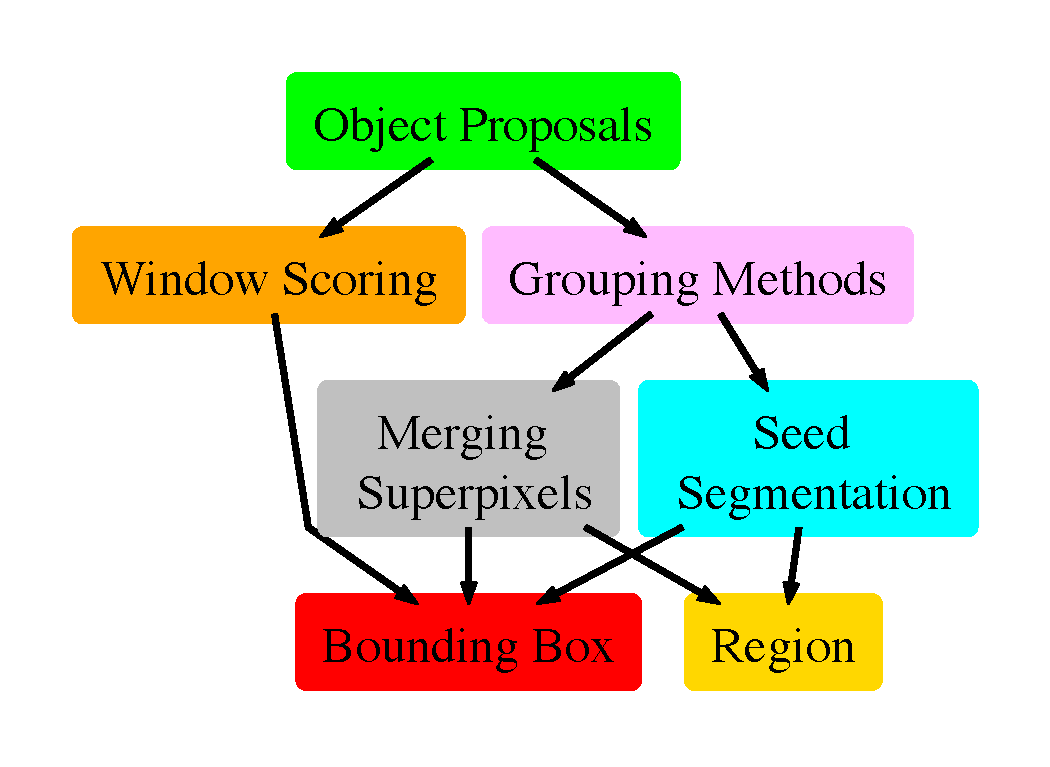
\includegraphics[width=0.5\textwidth]{figs/taxonomy.pdf}
\caption{A flowchart of how object proposals methods are organized depending on their scheme and localization. }
\label{fig:taxonomy}
\end{figure}

\subsection{Window Scoring Object Proposal}
\label{sec:window_scoring}
These methods try to directly differentiate objects within an image from background clutter. A common pipeline, is to start with an initial pool of candidate bounding boxes, then sort them according to some ranking model based on bottom-up image cues, and finally output the top few proposals. The second stage of the pipeline, the ranking model and its associated cues, represents the major differentiation between various methods within this sub-type.

{\bf Objectness}~\cite{Alexe:etal:PAMI12} is one the earliest works in the field. The method proposes an \emph{objectness} measure to score randomly-sampled image windows. The measure is based on multiple cues such as color, edge, and location. The most novel cue from this work is the ``superpixel straddling'' cue. Given a candidate bounding box this cue looks at the ratio of superpixel wholly contained within the window versus those superpixels intersecting the bounding box (straddling). The authors observe that this cue is strongly correlated to the presence or absence of an object in a candidate window. Finally, the localization of the output object proposals is limited to a bounding box. All subsequent methods can be seen as variants of \emph{objectness}.

A more recent set of papers  {\bf Bing}~\cite{Cheng:etal:CVPR14}, {\bf EdgeBoxes}~\cite{Zitnick:Dollar:ECCV14}, and {\bf ContourBox}~\cite{Lu:etal:ICCV15} have all focused their objectness measure exclusively on edge and/or contour cues. {\bf Bing} proposes a new cue based on the norm of gradients. The paper observes that generic objects exhibiting well-closed boundaries can be discriminated by measuring the norm of gradients. {\bf EdgeBoxes} generate object bounding box proposals using the primary cue of edge and contour content. This paper observes that the number of contained contours, grouped set of edgels, within a bounding box strongly correlates with the presence of an object. The scoring function is based on measuring the ratio of Structured Forest Edges~\cite{Dollar:Zitnick:PAMI15} within a bounding box that do and do not participate in contour formation. The approach of {\bf ContourBox} proposes a new cue based strictly on contour content. The authors observe that if a random window contains a semantic object then it most likely contains a closed contour and that contour tightly borders the bounding box. This is closely related to ``superpixel straddling'' but is based on edges rather than superpixels. Interestingly enough, though this method could output a closed contour, it does not and defaults to the standard bounding box for localization. Despite focusing on just edge/contour cues these methods are some of the most state of the art approaches, and more over they are very fast, as {\bf Bing} and {\bf EdgeBoxes} achieve near real-time performance.
 
While most of the methods have focused on improving the scoring function solely, other methods have also tried to improve other stages of the pipeline. {\bf Rahtu}~\cite{Rahtu:etal:ICCV11}  proposes new strategies to generate the initial set of bounding boxes along with an improved scoring function. Where as most methods start with a random or dense sampling of image windows, {\bf Rahtu}~\cite{Rahtu:etal:ICCV11} fits bounding boxes to individual superpixels and their combinations to generate a subset of initial windows. Another set of initial windows is generated by intelligently sampling from a learned prior on the discretized space of bounding boxes \ie $(x,y,w,h)$. An improved objectness measure which integrates new superpixel and edge cues is then utilized to score each window. {\bf MTSE}~\cite{Chen:etal:CVPR15}  like {\bf Rahtu} starts with an initial set of windows obtained by superpixels.  The paper also proposes a new cue ``superpixel tightness'' which measures how tight a bounding box adheres to an object. This cue can be seen as improvement on ``superpixel straddling'' by {\bf objectness}. By allowing varying degrees of tightness the localization error can be controlled and a wide diversity of object proposals can be generated. Finally, {\bf Zhang}~\cite{Zhang:Torr:PAMI16} proposed no new cues, but rather focused on improving the scoring strategy using simple gradient features. Rather than score each candidate bounding box in one step this paper proposes a two step procedure utilizing a cascade or ranking SVMs. The benefit of this approach is that rather than learn one general SVM for all bounding box scales, specific SVM can be learned be for each quantized scale and aspect ratio, and then calibrated in a second step. It is unclear how generalizable this approach is due to the large amount of learning on specific datasets.

Another closely related discipline is the area of detecting visual saliency. Various approaches have tried to combine saliency and objectness,  {\bf Objectness+Saliency}~\cite{Chang:etal:ICCV11}, or exclusively use saliency, {\bf Feng}~\cite{Feng:etal:ICCV11}, as a way to detect candidate object proposals. The method of  {\bf Objectness+Saliency} utilizes the objectness measure~\cite{Alexe:etal:PAMI12} coupled with saliency maps to score a randomly sampled set of image windows. There are no new cues proposed in this work compared to {\bf objectness}, but rather the integration of objectness and saliency is shown to improve both saliency maps and output bounding box object proposals. {\bf Feng}  correlates the presence of objects with visually salient portions of the image. Unlike~\cite{Chang:etal:ICCV11} which integrates objectness like cues, the authors only use a newly proposed window saliency measure. Window saliency is defined as the cost of composing the window using the remaining parts of the image. This measure is incorporated into a standard sliding window framework.
   
The {\bf objectness} framework is not limited to still images. {\bf SEEDS}~\cite{Bergh:etal:ICCV13} and {\bf Action Proposals}~\cite{Yu:etal:CVPR15} extend the generic idea to video. {\bf SEEDS} outputs a set of volumetric proposals that roughly corresponds to rectangular tubes sampled across frames.  The authors score each of these randomly sampled cuboids by adding a volumetric extension to the ``superpixel straddling'' cue from {\bf objectness}. The authors only use superpixels in their scoring function and they observe that multiple superpixel maps of various partition sizes greatly improves the results. {\bf Action Proposals}~\cite{Yu:etal:CVPR15} is similar to {\bf SEEDS} in that it outputs a temporal series of spatial bounding boxes, but this paper does not focus on general video but rather human action sequences. The authors score individual bounding boxes by a score similar to  {\bf objectness} called \emph{actionness}, that incorporates motion and appearance attributes consistent with human motion. After retaining bounding boxes of high ``actionness'' the authors utilize a max sub-path search algorithm to output the top-$N$ maximal ``actionness'' paths. 

While most image and video based methods follow the general pipeline of starting with an initial set of bounding boxes and scoring them, certain methods do not fit this traditional framework. {\bf Orient OP}~\cite{He:Lau:ICCV15} attaches an objectness score to each pixel rather than window. By operating at the pixel level each image gets turned into a likelihood map, which is then amenable to fitting bounding boxes of various orientations. Given an objectness per pixel the authors then adopt a mean-shift like procedure to fit a set of ellipses that correspond to regions exhibiting high likelihood. This makes the method better able to cope with non-rigid objects. The localization of the output object proposals is a set of oriented bounding boxes.


%% Structured Forest Edges[Cite this] are grouped into contours, and the authors observe that the number of wholly

%% A closely related approach 
%%  

%% \item 

%% \item {\bf Zhang}~\cite{Zhang:Torr:PAMI16} utilizes a cascade of ranking SVMs on simple gradient features. In the first stage, separate linear SVMs are learned for each quantized scale and aspect ratio. In the second stage, a ranking SVM is learned that calibrates the scoring function across all proposals from the first stage. Unlike the previous methods, this approaches proposes no new cues, but rather its contribution is in the scoring function. It is unclear how generalizable this approach is due to the large amount of learning on specific datasets. 

%% \item {\bf Rahtu}~\cite{Rahtu:etal:ICCV11} unlike other \emph{window-scoring} methods makes improvements not only to the scoring function but also proposes new strategies to generate the initial set of bounding boxes. Where as most methods start with a random or dense sampling of image windows, ~\cite{Rahtu:etal:ICCV11} uses superpixels and their combinations to generate a subset of initial windows. Another set of initial windows is generated by intelligently sampling from a learned prior on the discretized space of bounding boxes \ie $(x,y,w,h)$. An improved objectness measure which integrates new superpixel and edge cues is then utilized to score each window. 

%% \item {\bf Bing}~\cite{Cheng:etal:CVPR14} adopts a sliding window framework and evaluates each of the windows using a simple linear classifier. The novel cue in this work, is based on looking at the norm of gradients. The paper observes that this features strongly correlates with objects exhibiting well-closed boundaries. Utilizing a binarized version of this cue for discrimination the authors are able to leverage a near real-time scheme. 

%% \item {\bf EdgeBoxes}~\cite{Zitnick:Dollar:ECCV14} generate object bounding box proposals using the primary cue of edge content. Structured Forest Edges[Cite this] are grouped into contours, and the authors observe that the number of wholly contained contours within a bounding box strongly correlates with the presence of an object. The scoring function is based on measuring the ratio of edges within a bounding box that do and do not participate in contour formation. Similar to Bing~\cite{Cheng:etal:CVPR14} this method achieves near real time performance. 
 
%% \item {\bf MTSE}~\cite{Chen:etal:CVPR15} proposes a new cue ``superpixel tightness'' which measures how tight a bounding box adheres to an object. By allowing varying degrees of tightness the localization error can be controlled and a wide diversity of object proposals can be generated. Finally, like Rahtu~\cite{Rahtu:etal:ICCV11} this method start with an initial set of windows obtained by superpixels. 

%% \item {\bf ContourBox}~\cite{Lu:etal:ICCV15} proposes a new cue based on contour content. The authors observe that if a random window contains a semantic object then it most likely contains a closed contour and that contour tightly borders the bounding box. These two constraints are combined into an objective function whose solution serves as an indicator of objectness. 

%% \item {\bf Orient OP}~\cite{He:Lau:ICCV15} attaches an objectness score to each pixel rather than window. By operating at the pixel level each image gets turned into a likelihood map, when then is amenable to fitting bounding boxes of various orientations. Given an objectness per pixel the authors then adopt a mean-shift like procedure to fit a set of ellipses that correspond to regions exhibiting high likelihood. The localization of the output object proposals is a set of oriented bounding boxes.

%% \end{itemize}

%% Another closely related discipline is the area of detecting visual saliency. The intuition behind this research area is that when a human subject observes an image his or her eyes are immediately fixated on certain items within the image that stand out amongst its surroundings. Rather than process the whole image, we should focus on these ``visually salient'' areas. The goal of an algorithm is to output a likelihood map that hopefully can predict these visually salient areas of an image as measured by human eye gaze patterns. These maps can then be used in various computer vision high level tasks. 

%% While both window scoring object proposal methods and visual saliency algorithms share the same high-level goal they differ in what is semantically meaningful and how to represent it. Windows scoring methods are looking for rectangular regions of the image that hopefully contain objects and represent this as a set of output bounding boxes. Where as visual saliency is concerned with transforming an image into a likelihood map which measures the importance of each pixel as it relates to human visual attention. An object may or may not exist in a visual saliency map and bounding box object proposals might not be visually salient.  Despite their differences, various window-scoring methods have been proposed~\cite{Chang:etal:ICCV11} that try to merge the concepts of objectness and saliency. 

%% \begin{figure*}[pht]
%% \centering
%% \begin{tabular}{|c|c|c|c|c|}
%% \hline
%% Method & Approach & Input & Output & Ranking \\
%% \hline
%% \multicolumn{5}{|c|}{2007}\\
%% \hline
%% Soup of Segments~\cite{Malisiewicz:Efros:BMVC07} & & & & \\
%% \hline
%% Shock Patch Fragments~\cite{Ozcanli:Kimia:BMVC07} & & & & \\
%% \hline
%% \multicolumn{5}{|c|}{2010}\\
%% \hline
%% Objectness~\cite{Alexe:etal:PAMI12}& & & & \\
%% \hline
%% CIP~\cite{Endres:Hoiem:PAMI14}& & & & \\
%% \hline
%% CPMC~\cite{Carreira:Sminchisescu:PAMI12}& & & & \\
%% \hline
%% \multicolumn{5}{|c|}{2011}\\
%% \hline
%% Objectness+Saliency~\cite{Chang:etal:ICCV11} & & & & \\
%% \hline
%% Rahtu~\cite{Rahtu:etal:ICCV11} & & & & \\
%% \hline
%% Zhang~\cite{Zhang:Torr:PAMI16} & & & & \\
%% \hline
%% Feng~\cite{Feng:etal:ICCV11} & & & & \\
%% \hline
%% Selective Search~\cite{Uijlings:etal:IJCV13} & & & & \\
%% \hline
%% \multicolumn{5}{|c|}{2012}\\
%% \hline
%% MVF~\cite{Narayanan:Kimia:ECCV12} & & & & \\
%% \hline
%% Shape Sharing~\cite{Kim:Grauman:ECCV12} & & & & \\
%% \hline
%% \multicolumn{5}{|c|}{2013}\\
%% \hline
%% RandomizedPrim~\cite{Manen:etal:ICCV13} & & & & \\
%% \hline
%% SEEDS~\cite{Bergh:etal:ICCV13} & & & & \\
%% \hline
%% \multicolumn{5}{|c|}{2014}\\
%% \hline
%% Spatio-Temp Proposals~\cite{Oneata:etal:ECCV14} & & & & \\
%% \hline
%% RIGOR~\cite{Humayun:etal:CVPR14} & & & & \\
%% \hline
%% MCG~\cite{Arbelaez:etal:CVPR14} & & & & \\
%% \hline
%% Rantalankila~\cite{Rantalankila:etal:CVPR14} & & & & \\
%% \hline
%% GOP~\cite{Krahenbuhl:Koltun:ECCV14} & & & & \\
%% \hline
%% Bonev~\cite{Bonev:Yuille:ECCV14} & & & & \\
%% \hline
%% EdgeBoxes~\cite{Zitnick:Dollar:ECCV14} & & & & \\
%% \hline
%% Bing~\cite{Cheng:etal:CVPR14} & & & & \\
%% \hline
%% DeepMultiBox~\cite{Erhan:etal:CVPR14} & & & & \\
%% \hline
%% \multicolumn{5}{|c|}{2015}\\
%% \hline
%% LPO~\cite{Krahenbuhl:Koltun:CVPR15} & & & & \\
%% \hline
%% Xiao~\cite{Xiao:Lu:etal:CVPR15} & & & & \\
%% \hline
%% Action Proposals~\cite{Yu:etal:CVPR15} & & & & \\
%% \hline
%% MTSE~\cite{Chen:etal:CVPR15} & & & & \\
%% \hline
%% CPMC RGB-D~\cite{Banica:Sminchisescu:CVPR15} & & & & \\
%% \hline
%% Video Proposals~\cite{Wu:etal:CVPR15} & & & & \\
%% \hline
%% Contour Box~\cite{Lu:etal:ICCV15} & & & & \\
%% \hline
%% POISE~\cite{Humayun:etal:ICCV15} & & & & \\
%% \hline
%% Orient OP~\cite{He:Lau:ICCV15} & & & & \\
%% \hline
%% \end{tabular}
%% \caption{XXX}
%% \label{fig:op_table}
%% \end{figure*}

\subsection{Grouping Based Method}
\label{sec:grouping_methods}
While window-based object proposals will generally suffice for representing roughly-rectangular objects such as bottles, mugs, and cars they are definitely not precise enough to represent more deformable objects such as animals or plants. To represent the latter one needs to capture the shape of the object as delineated by a segmented binary mask. \emph{Grouping based} proposal methods refer to all methods that attempt to generate multiple (possibly overlapping) segments that are likely to correspond to objects. Within grouping based methods two distinct paradigms have emerged for how to generate these proposals. Candidate object proposals can either be produced by \emph{merging superpixels} according to various heuristics or by generating multiple foreground-background segmentations for various seed regions, \emph{seed segmentation}. Irrespective of approach \emph{all} grouping-based schemes enjoy the strength of localizing output object proposals by either a segmentation mask and/or a bounding box. 
\newline
\newline
\noindent
{\bf Merging Superpixels:} This approach is most closely associated with traditional region-based segmentation. In fact the simplest approach is to take any image segmentation algorithm or superpixel partitioning and treat each non-overlapping segment as an independent object proposal. While this approach is valid, the likelihood of finding an object proposal is severely limited to a single pool of candidates generated by a greedy bottom-up grouping process. To increase the likelihood of finding meaningful object proposals, we need to diversify the number and type of candidates that we consider. It is exactly this diversification step that differs among various methods. 


The {\bf Soup of Segments}~\cite{Malisiewicz:Efros:BMVC07} approach by Malisiewicz \etal represents one of the earliest papers on generating region-based object proposals. Rather than explore a single segmentation, the author's generate a pool of candidate proposals by first running multiple segmentation algorithms with varying parameters. Given this initial pool of regions the approach further diversifies the pool by adding proposals obtained by merging adjacent segments. Roughly around that same time, the object recognition work by Gu \etal~\cite{Gu:etal:CVPR09} utilized a single segmentation algorithm, gPb-owt-ucm~\cite{Arbelaez:etal:PAMI11}, but diversified the solution space by utilizing segments at all levels of the hierarchal region tree. One of the most state of the art methods, {\bf Multi-Scale Combinatorial Grouping (MCG)}~\cite{Arbelaez:etal:CVPR14} diversifies the space further by exploring segmentations across multiple scales. The algorithm runs the gpb-owt-ucm~\cite{Arbelaez:etal:PAMI11} algorithm at three different scales, and the region hierarchies are then aligned across scales into one unified region hierarchy. Regions within this integrated hierarchy serve as one set of object proposals. Similar to the soup of segments approach {\bf MCG} extends the pool of candidates further by considering combinations of regions across various levels of the multi-scale hierarchy. Empirically this work determined that the optimum combination is a triplet, and anything beyond that only leads to marginal improvements. The approach of {\bf Bonev} \etal~\cite{Bonev:Yuille:ECCV14} adopts a similar approach but the hierarchy is generated using a PageRank like dissimilarity measure of SLIC~\cite{Achanta:etal:PAMI12} superpixels. Identical to MCG the algorithm forms triplets by selecting a subset of segments from the more coarse levels of the hierarchy.

 %%  \emph{It is important to realize that the output localization is not what differentiates various methods but rather the process by which the object proposals are formed in the first place}. 


The previous methods~\cite{Malisiewicz:Efros:BMVC07,Arbelaez:etal:CVPR14,Bonev:Yuille:ECCV14} aim to provide precise pixel level object delineation where as an alternative set of grouping methods attempt to provide rough object locations in the form of bounding boxes. Among methods of this type the most broadly used is {\bf Selective Search}~\cite{Uijlings:etal:IJCV13} which is currently the method of choice for many of the state of the art object detectors, R-CNN~\cite{Girshick:etal:PAMI16}. Similar to previous methods {\bf Selective Search} generates a hierarchal segmentation by greedily merging pairs of regions according to a similarity measure based on size and texture features. The process terminates when the image becomes a single region. To diversify the space further a region tree is computed independently for various color-spaces. The final output is a bounding box for each region at all levels of the hierarchy for the various color spaces. The approach of {\bf Xiao} \etal~\cite{Xiao:Lu:etal:CVPR15} adopts the same grouping scheme, but introduces a new approach to measure superpixel compatibility. Rather than pick one global distance, the distance adapts locally to the underlying image complexity. The output like {\bf Selective Search} is a set of bounding boxes. {\bf RandomizedPrim}~\cite{Manen:etal:ICCV13} adopts similar features to~\cite{Uijlings:etal:IJCV13} but rather than generate a hierarchy of segments it adopts the popular graph based segmentation framework. Given a weighted region-adjacency graph the problem of proposal generation is treated as the sampling of connected subgraphs that maximize edge weights. The authors generate random sub-trees by utilizing a stochastic version of prim's algorithm with the output being a set of fitted bounding boxes to each superpixel subgraph. 

The previous methods~\cite{Uijlings:etal:IJCV13,Xiao:Lu:etal:CVPR15,Manen:etal:ICCV13} output bounding boxes object proposals despite being able to produce object level masks. While the outputs are identical, these methods should {\bf not} be considered window-scoring as the object proposal generation step is not based on sampling a set of random windows, but rather on merging superpixels whose \emph{output} just happens to be a bounding box. Furthermore, no type of window scoring is applied by these methods to the output bounding box proposals. 

Finally, the approach of grouping superpixels to generate object proposals has also been extended to video. In video applications, the goal is to produce a small set of supervoxels or volumetric proposals that correspond to objects exhibiting high temporal or appearance consistency across many frames. The work of {\bf Spatio-Temporal Proposals}~\cite{Oneata:etal:ECCV14} extends the work of {\bf RandomizedPrim}~\cite{Manen:etal:ICCV13} to video.  {\bf Spatio-Temporal Proposals} initially constructs a region adjacency graph of SLIC~\cite{Achanta:etal:PAMI12} superpixels for each individual frame, and then the graphs are connected across all frames to produce a three-dimensional superpixel graph for the whole video. Once the superpixel graph is computed agglomerate clustering is run to produce a hierarchal tree of supervoxels. Finally, given this supervoxel tree the method adapts the approach of {\bf RandomizedPrim} to produce a set of randomized supervoxels and their combinations that maximizes some measure of spatial and temporal appearance consistency.
\newline
\newline
\noindent
{\bf Seeded Segmentation:} These approaches can trace their roots back to interactive segmentation techniques like GrabCut~\cite{Rother:etal:GRAPHICS04}. Given an user annotated foreground region and background region these interactive techniques utilize the seed statistics to segment the object from the background. We can adapt these interactive techniques to generate multiple segmentations by rerunning the process with varying seed placement, size, or shape. Methods that fall under this umbrella essentially are automating this procedure.

The two earliest works that adopt this approach are Constrained Parametric Min-Cuts ({\bf CPMC})~\cite{Carreira:Sminchisescu:PAMI12} and Category Independent Proposals ({\bf CIP})~\cite{Endres:Hoiem:PAMI14}. In {\bf CPMC}, a large number of independent binary min-cut segmentation problems are solved by starting from a sampling of foreground and background seeds with varying degrees of foreground bias. The pool of object candidates is further diversified by varying foreground seed size, shape, and placement in various combinations with background seeds. {\bf CIP} samples a set of seed regions, obtained from a hierarchical segmentation and by varying parameters in a CRF framework, generates a diverse set of regions that are guided toward object segmentations by learned affinity functions. The biggest difference between the two methods is that {\bf CPMC} operates at the pixel level while {\bf CIP} operates at the superpixel level. Other methods within this domain can be seen as variants of these two approaches. 

{\bf Rigor}~\cite{Humayun:etal:CVPR14} drastically improves the computationally efficiency of {\bf CPMC} in two ways. The authors observe that many combination of seed parameters lead to redundant computations. By capturing this computation in the form of a graph it can be reused across multiple graph-cut problems. Secondly, {\bf RIGOR} operates on a superpixel graph compared to the pixel graph used in previous methods. {\bf POISE}~\cite{Humayun:etal:ICCV15} observes that {\bf CPMC} tends to produce objects which are either comparable in size to the seed region or extend almost to the full image. Medium sized objects which do not exist at these extremes, seed scale or image scale, are frequently missing in the generated pool of candidates. To overcome this ``middle child'' problem POISE augments the energy minimization framework of {\bf CPMC} with the signed geodesic distance. The new framework facilitates the formation of medium-sized objects by lowering the energy needed to solve the objective function. Overall, seeded segmentation approaches based on graph-cuts based tend to produce the most accurate object proposals when compared to region-based merging methods, but this accuracy comes at the expense of increased computational run-times. 

While most seed-based methods utilize the underlying graph-cut technology to perform the actual segmentation, some methods do not. Geodesic Object Proposal ({\bf GOP})~\cite{Krahenbuhl:Koltun:ECCV14} is  similar to other graph-cut approaches in that it is based on seed based segmentation, but how it uses the seeds and performs the segmentation differs drastically. Each seed is a superpixel and the optimal placement of background/foreground seeds is learned rather than the uniform sampling of CPMC. Furthermore, rather than utilize each seed directly in a graph-cut formulation the foreground/background seeds are dilated into binary masks according to some learned process. A Signed Geodesic distance transform is computed for these masks, and the critical level sets define a set of figure/ground segmentations which serve as the output object proposals. Similar to CPMC the pool of object proposals is increased by considering various superpixel foreground/background learned seed placements in the image.

Finally, seeded segmentation approaches have been extended to video and depth images. {\bf Video Proposals} by Wu \etal~\cite{Wu:etal:CVPR15} proposed a scheme based on {\bf RIGOR} proposals to generate a set of volumetric video proposals. Object proposals are extracted independently for each frame, and optimizing over all possible tracks those that exhibit high appearance and temporal consistency are output as the final set of volumetric proposals. The paper focuses on generating video proposals that are robust to occlusion which is much more of a problem in a video sequence than for a single image. The work of CPMC was extended to depth images, {\bf CPMC-RGBD}~\cite{Banica:Sminchisescu:CVPR15}. In {\bf CPMC-RGBD} the pairwise term of the energy function is augmented to not only measure the spatial consistency of image $gPb$ values, but also the $gPb$ probabilities across the depth channel. These proposals are then utilized for semantic segmentation of depth images. 

While many methods fit into one of these two sub-types, certain methods while still grouping based cannot be classified as purely superpixel merging or purely seed-based segmentation. The approach of {\bf Rantalankila} \etal ~\cite{Rantalankila:etal:CVPR14} is a hybrid method that proposes a superpixel merging strategy similar to {\bf SelectiveSearch} but couples that with a {\bf CPMC} like refinement. For each level of the hierarchy the generated regions are used as foreground/background seeds to solve multiple graph cuts which increases the pool of proposals to consider. Unlike {\bf SelectiveSearch} the output is a segmentation mask instead of a bounding box.  

\subsection{Other Methods}

While the vast majority of object proposal methods are either window-scoring or grouping based there are some approaches that do not fit into either. Characteristic of all these methods is that they do not focus on solely bottom-up processing but rather incorporate top-down cues or utilize a more learned approach. {\bf Shape Sharing}~\cite{Kim:Grauman:ECCV12} proposes a top-down bottom up approach to generate object proposals. The method fits a set of exemplars in the form of object level silhouettes to low-level edge content. The fitted shapes are then further refined using graph cuts.  {\bf DeepMultiBox}~\cite{Erhan:etal:CVPR14} shares some similarity with window-scoring methods but rather than adopt a sliding window framework, the system trains a neural network to directly predict a fixed number of bounding box proposals. {\bf Learning to Propose Objects} (LPO)~\cite{Krahenbuhl:Koltun:CVPR15} looks at the formation of region based object proposals as a problem of ensemble learning. The key idea is that rather than vary parameters to generate a wide variety of proposals, the same can be achieved by learning over many individual figure-ground segmentation models.  Both {\bf DeepMultiBox} and {\bf LPO} can be seen as treating \emph{window-scoring} and \emph{grouping-based methods} as supervised learning problems respectively. 

%The field can be summarized in~\ref{fig:op_table}

\subsection{Ranking Proposals}

A common problem that arises when utilizing object proposals, is how to retain a fixed number of proposals? In many cases, top level applications such as object recognition and video segmentation are limited computationally to a fixed set of candidates that they can process. Another motivation is that when evaluating multiple algorithms that produce a varying number of candidates it would be beneficial to look at their performance at a fixed number of proposals. This problem has been traditionally treated as a ranking problem where by the goal is to retrieve the top $N$ proposals that highly correlate with objects out of a much larger pool. While this is a worthwhile goal in its own right, the ranking or scoring object proposals is {\bf not} a requirement for an object proposal method.

All window scoring methods inherently have the ability to rank proposals. A user utilizing one of these algorithms can recall the top 10, top 100, or any fixed $N$. Along with their speed, this represents their greatest advantage over grouping methods. This does not mean that grouping methods do not have a ranking like procedure. The methods of {\bf CIP}~\cite{Endres:Hoiem:PAMI14} and {\bf CPMC}~\cite{Carreira:Sminchisescu:PAMI12} proposed a generic ranker based on bottom-up images features that produces a diverse set of solutions \ie proposals of various size and at different locations should be in the top $K$. Despite different formulations of the ranking problem, these two methods use similar cues and also overlap with many of the cues utilized in objectness. MCG~\cite{Arbelaez:etal:CVPR14} adopts the same type of ranker as CPMC~\cite{Carreira:Sminchisescu:PAMI12}. Other methods such as Geodesic Object Proposal (GOP)~\cite{Krahenbuhl:Koltun:ECCV14}, LPO~\cite{Krahenbuhl:Koltun:CVPR15}, Rantalankila~\cite{Rantalankila:etal:CVPR14}, and RIGOR~\cite{Humayun:etal:CVPR14} do not have a ranker. Of course, it is trivial to attach any ranking scheme to any grouping based method by either reutilizing existing schemes such as the {\bf CPMC} ranker or {\bf CIP}, or treating each segmented proposal as a bounding box and using the {\bf objectness} score. Finally, while all rankers irrespective of approach try to produce generic object candidate rankers it is not clear how general they are, as the majority of rankers are trained on various versions of the VOC datasets.

\subsection{Our Work}

Our approach can be classified as a \emph{grouping method}. While we fall under this umbrella, our approach differs drastically from other methods in three major aspects , \emph{(i)} representation \emph{(ii)}, approach, and \emph{(iii)} level of localization. 

Most methods irrespective of subtype, seed segmentation or merging superpixels, either utilize Felzenszwalb and Huttenlocher (FH)~\cite{Felzenszwalb:Huttenlocher:IJCV04} or SLIC~\cite{Achanta:etal:PAMI12} superpixels. While these regional representations capture the appearance based characteristics of objects in an image, they fail to capture the other important cue, namely contours. As recent window-scoring papers have shown,~\cite{Cheng:etal:CVPR14,Zitnick:Dollar:ECCV14,Lu:etal:ICCV15}, edge/contour content is a very discriminative cue for determining an object. Regional schemes try to capture this, by utilizing the \emph{gPb} probability, but we incorporate this information explicitly in the form of an ordered set of edgels. However, while contours bring out cues that appearance is missing, we still need to incorporate regional information as our goal is an accurate pixel-level object delineation.  To achieve this we motivate and adopt a layered representation based on the medial axis that is neither purely regional based or contour based, but rather is an intermediate level representation that allows us to effectively output segmented proposals while reasoning with both types of cues. 

The second major differentiation is our approach to diversify the space of object proposals.  For example, given a superpixel representation we can generate different object proposals by varying the levels of the region hierarchy or dendrogram, the number of superpixels at each level, and finally the cardinality of our merging step i.e. pairs, triplets, or quads. Each object proposal is then parameterized by one combination of these parameters and we can generate a set of object proposals by sweeping this parameter space. The same can be said for graph cut methods where the seed shape, seed location, seed size, and bias between energy terms are sufficiently discretized and swept to diversify the set of output object proposals. In our work we deviate drastically from this ``regions by parameter sweeping'' approach by adopting a more structured and exhaustive methodology where by we look at the formation of a single object proposal not as merely a particular permutation of input parameters but rather as the result of a reorganization of an image. 

Finally, while all grouping methods, output a region, we argue for another level of localization, namely the contour bounding the object. While in the case of closed regions there is a duality between the contour and region, the same cannot be said for non-closed regions. These non-closed regions are predominantly associated with parts but more over occur when an object is being occluded. The contour provides a clue that this region is a ``part-of'' something than a whole independent object. 

%% We extend our evaluation to not only measure how well our object proposals agree with ground-truth segmentation but also how well our contours map to user-annotated silhouettes.


\subsection{Medial Axis Work}


There is limited work in the computer vision community on utilizing the shock graph/medial axis for object proposal generation. Most of the prior uses of the medial axis have focused on utilizing the representation solely for perceptual organization. The first paper to propose using the shock graph for perceptual organization was by Tek and Kimia~\cite{Tek:Kimia:CVPR99}. This theoretical paper proposed that the shock graph is an appropriate intermediate level representation for organizing the shape (contours) by way of a set of transforms (graph operations) of the underlying shock graph. An extension of this work~\cite{Johannes:POCV2001}, proposed a computational algorithm for realizing this vision. However, both papers were theoretical in nature and even more importantly only considered transformations of the shock graph affecting the contour map. 

The idea of utilizing the shock graph to organize the image was proposed in the mid 2000s by two different papers, {\bf Shock Patch Fragments} by Ozcanli \etal~\cite{Ozcanli:Kimia:BMVC07} and Tamrakar \etal~\cite{Tamrakar:Kimia:POCV04}. In {\bf Shock Patch Fragments}, the shock graph was treated in a similar manner to seeded-region growing methods, by expanding out depth-first indiscriminately from a set of nodes. These sub-graphs were then shown to effectively decompose the image into a set of parts, (horse heads, horse legs, etc). However, this approach had similar problems to standard segmentations method as it assumed a pristine contour map and hence a perfect shock graph. The latter work built upon~\cite{Tek:Kimia:CVPR99} and argued that the shock graph is an appropriate mid-level representation to not only perceptually organize the contour map, but also to segment the image. However, it proposed only a theoretical framework to achieve this and was in more line with the segmentation paradigm of that time. Our approach effectively builds on that idea in the context of producing object proposals. 

The current work in the medial axis community most related to ours is the work by Lee \etal~\cite{Lee:Fidler:Dickinson:ICCV13}. This work can be classified as a \emph{grouping method} based on merging superpixels with the output localization being a region. This paper focuses on generating part-level proposals which has received considerably less attention than object level proposals. Parts are segmented in a bottom-up manner by taking advantage of the property that most real-world parts exhibit symmetry. By treating each superpixel as a deformable disc, a part constitutes a chain of these discs, or equivalently a set of merged superpixels that maximizes some measure of symmetry. We differ in two important ways from this work. One, our method produces full object proposals along with part proposals. Two, is in how the medial axis is used. In the work of~\cite{Lee:Fidler:Dickinson:ICCV13} the authors do not directly utilize the medial axis as they argue it is amenable only to closed shapes and instead approximate the medial axis branches with the locus of superpixel centers. In our approach we transform the image directly into a shock graph representation, medial axis refinement, by taking advantage of an advanced new shock computation algorithm,~\cite{Tamrakar:Kimia:Shock}.

%% The resulting pool of figure segments are then processed and ranked using certain regularities typical of projections of real-world objects, and a learning scheme is used to sample a diverse subset. 

%% Another recent paper
%% \cite{Endres:Hoiem:ECCV10} a structured learning approach is then used to rank the regions so that the top-ranked regions are likely to correspond to different objects.



%% 


%% Selective Search~\cite{Uijlings:etal:IJCV13}, RandomizedPrim~\cite{Manen:etal:ICCV13}

 
%% \begin{figure}[ht]
%% \centering
%% 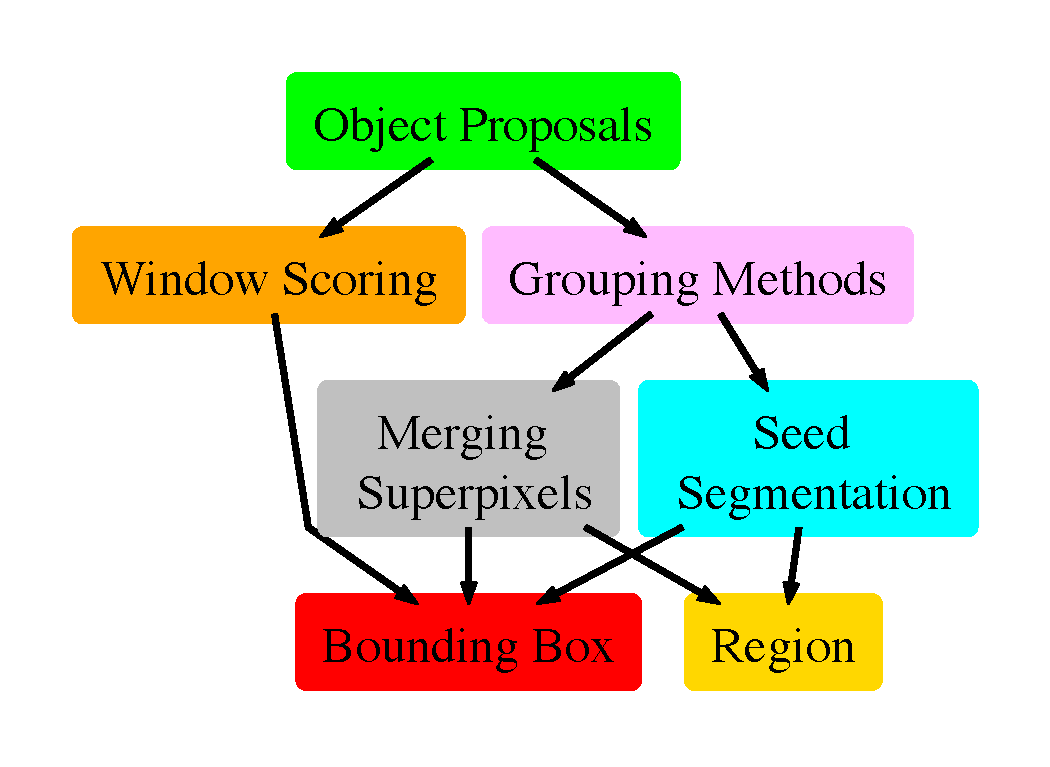
\includegraphics[width=0.5\linewidth]{figs/taxonomy.pdf}
%% \caption{XXX}
%% \label{fig:taxonomy}
%% \end{figure}

%% 

